\documentclass{article}

% Required packages
\usepackage{amssymb}
\usepackage{amsmath}
\usepackage{graphicx}
\usepackage{geometry}
\usepackage{tikz}
\usepackage{array}
\usepackage{booktabs}
\usepackage{enumitem}
\usepackage{listings}
\usepackage{xcolor}

% Set page geometry
\geometry{a4paper, margin=1in}

% Configure listings for Python
\lstset{
  language=Python,
  basicstyle=\ttfamily\footnotesize,
  numbers=left,
  numberstyle=\tiny\color{gray},
  frame=single,
  breaklines=true,
  breakatwhitespace=true,
  captionpos=b,
  tabsize=4,
  showspaces=false,
  showstringspaces=false,
  showtabs=false,
  commentstyle=\color{gray}\textit,
  keywordstyle=\color{blue}\bfseries,
  stringstyle=\color{red}
}

% For centering images and tables
\usepackage{float}

\begin{document}

\begin{flushright}
   Randall Rogers\\
   DSC 255: Machine Learning Fundamentals\\
   Homework 3 \\
   Spring 2025 \\
\end{flushright}

\subsection*{Question 1}
\parbox{\textwidth}{Gaussian parameters. Each of the following scenarios describes a joint distribution $(x, y)$. In each case, give the parameters of the (unique) bivariate Gaussian that satisfies these properties.}

\begin{enumerate}[label=(a)]
    \item x has mean 2 and standard deviation 1, y has mean 2 and standard deviation 0.5, and the
correlation between x and y is -0.5.
\end{enumerate}
\begin{enumerate}[label=(b)]
    \item x has mean 1 and standard deviation 1, and y is equal to 2.
\end{enumerate}

\parbox{\textwidth}{\textbf{Solution (a)}}

\noindent\rule{\textwidth}{0.4pt}\\
\parbox{\textwidth}{For a bivariate Gaussian distribution, we need to specify the following parameters:}\\

$$\boldsymbol{\mu} = [\mu_x, \mu_y]^T$$\\
$$\boldsymbol{\Sigma} = \begin{bmatrix} \sigma_x^2 & \rho\sigma_x\sigma_y \\ \rho\sigma_x\sigma_y & \sigma_y^2 \end{bmatrix}$$

\begin{itemize}
    \item Mean vector: $\boldsymbol{\mu}$
    \item Covariance matrix: $\boldsymbol{\Sigma}$
\end{itemize}

\parbox{\textwidth}{Let $\mu_x = 2$, $\mu_y = 2$, $\sigma_x = 1$, $\sigma_y = 0.5$, and $\rho = -0.5$}\\

\parbox{\textwidth}{Solve for mean vector $\boldsymbol{\mu}$:}\\

$$\boldsymbol{\mu} = \begin{bmatrix} \mu_x & \mu_y \end{bmatrix}^T = \begin{bmatrix}
    \mu_x \\
    \mu_y
\end{bmatrix} = \begin{bmatrix}
    2 \\
    2
\end{bmatrix}$$\\

\parbox{\textwidth}{Solve for covariance matrix $\boldsymbol{\Sigma}$:}\\

$$\boldsymbol{\Sigma} = \begin{bmatrix} \sigma_x^2 & \rho\sigma_x\sigma_y \\ \rho\sigma_x\sigma_y & \sigma_y^2 \end{bmatrix} = \begin{bmatrix} 1^2 & (-0.5)(1)(0.5) \\(-0.5)(1)(0.5) & 0.5^2\end{bmatrix} = \begin{bmatrix} 1 & -0.25 \\-0.25 & 0.25\end{bmatrix}$$\\

\parbox{\textwidth}{$\therefore$ the bivariate Gaussian has parameters:}\\

$$\mathcal{N}\left(\begin{bmatrix} 2 \\ 2 \end{bmatrix}, \begin{bmatrix} 
    1 & -0.25 \\
    -0.25 & 0.25
\end{bmatrix}\right)$$

\noindent\rule{\textwidth}{0.4pt}\\

\newpage

\parbox{\textwidth}{\textbf{Solution (b)}}

\noindent\rule{\textwidth}{0.4pt}\\

\parbox{\textwidth}{For a bivariate Gaussian distribution, we need to specify the following parameters:}\\

$$\boldsymbol{\mu} = [\mu_x, \mu_y]^T$$\\
$$\boldsymbol{\Sigma} = \begin{bmatrix} \sigma_x^2 & \rho\sigma_x\sigma_y \\ \rho\sigma_x\sigma_y & \sigma_y^2 \end{bmatrix}$$

\begin{itemize}
    \item Mean vector: $\boldsymbol{\mu}$
    \item Covariance matrix: $\boldsymbol{\Sigma}$
\end{itemize}

\parbox{\textwidth}{Let $\mu_x = 1$, $\mu_y = 2$, $\sigma_x = 1$, $\sigma_y = 0$}\\

\parbox{\textwidth}{Solve for mean vector $\boldsymbol{\mu}$:}\\

$$\boldsymbol{\mu} = \begin{bmatrix} \mu_x & \mu_y \end{bmatrix}^T = \begin{bmatrix}
    \mu_x \\
    \mu_y
\end{bmatrix} = \begin{bmatrix}
    1 \\
    2
\end{bmatrix}$$\\

\parbox{\textwidth}{Solve for covariance matrix $\boldsymbol{\Sigma}$:}\\

$$\boldsymbol{\Sigma} = \begin{bmatrix} \sigma_x^2 & \rho\sigma_x\sigma_y \\ \rho\sigma_x\sigma_y & \sigma_y^2 \end{bmatrix} = \begin{bmatrix} 1^2 & 0 \\ 0 & 0^2\end{bmatrix} = \begin{bmatrix} 1 & 0 \\ 0 & 0\end{bmatrix}$$\\

\parbox{\textwidth}{$\therefore$ the bivariate Gaussian has parameters:}\\

$$\mathcal{N}\left(\begin{bmatrix} 1 \\ 2 \end{bmatrix}, \begin{bmatrix} 
    1 & 0 \\
    0 & 0
\end{bmatrix}\right)$$

\noindent\rule{\textwidth}{0.4pt}\\

\noindent\rule{\textwidth}{0.4pt}\\

\newpage
\subsection*{Question 2}
\parbox{\textwidth}{A generative approach is used for a binary classifcation problem (with classes +, -) and it turns out
that the resulting classifier predicts + at all points x in the input space. Why might this be?}\\

\parbox{\textwidth}{\textbf{Solution}}
\noindent\rule{\textwidth}{0.4pt}\\

\parbox{\textwidth}{\textbf{Step 1:} Recall the Bayesian decision rule for generative classifiers.}

\vspace{0.2cm}

\parbox{\textwidth}{In a generative approach, we model the joint distribution $p(x, y)$ by learning the class-conditional densities $p(x|y)$ and prior probabilities $p(y)$. The classification decision is made using Bayes' rule:}

$$\hat{y} = \arg\max_{y \in \{+,-\}} p(y|x) = \arg\max_{y \in \{+,-\}} \frac{p(x|y)p(y)}{p(x)}$$

\parbox{\textwidth}{Since $p(x)$ is constant for both classes, the decision rule simplifies to:}

$$\hat{y} = \arg\max_{y \in \{+,-\}} p(x|y)p(y)$$

\vspace{0.3cm}

\parbox{\textwidth}{\textbf{Step 2:} Analyze the decision boundary.}

\vspace{0.2cm}

\parbox{\textwidth}{For binary classification, we predict the positive class (+) when:}

$$p(x|+)p(+) > p(x|-)p(-)$$

\parbox{\textwidth}{Equivalently, taking the logarithm (which preserves the inequality since log is monotonically increasing):}

$$\log p(x|+) + \log p(+) > \log p(x|-) + \log p(-)$$

\vspace{0.3cm}

\parbox{\textwidth}{\textbf{Step 3:} Identify possible reasons for always predicting the positive class.}

\vspace{0.2cm}

\parbox{\textwidth}{There are several reasons why the inequality $p(x|+)p(+) > p(x|-)p(-)$ might hold for all $x$:}

\begin{enumerate}
    \item \textbf{Highly imbalanced prior probabilities:} If $p(+) \gg p(-)$, the classifier might always predict the positive class because the prior term dominates the decision, regardless of the likelihood term. This occurs when the training data contains many more positive examples than negative ones.
    
    \item \textbf{Poor estimation of class-conditional densities:} If $p(x|+)$ is consistently overestimated or $p(x|-)$ is consistently underestimated across the input space, the classifier will favor the positive class.
    
    \item \textbf{Model misspecification:} If the assumed parametric form of $p(x|y)$ (e.g., Gaussian) does not match the true distribution of the data, the estimated densities may lead to systematic classification errors.
    
    \item \textbf{Feature insufficiency:} If the selected features do not provide discriminative information to separate the classes, the model might default to the more common class.
    
    \item \textbf{Numerical issues:} In high-dimensional spaces, numerical underflow when computing likelihoods can lead to computational issues that affect the decision boundary.
\end{enumerate}

\vspace{0.3cm}

\parbox{\textwidth}{\textbf{Step 4:} Mathematical illustration with Gaussian class-conditionals.}

\vspace{0.2cm}

\parbox{\textwidth}{For a concrete example, consider a generative classifier with Gaussian class-conditionals:}

$$p(x|+) \sim \mathcal{N}(\mu_+, \Sigma_+)$$
$$p(x|-) \sim \mathcal{N}(\mu_-, \Sigma_-)$$

\parbox{\textwidth}{The decision boundary is determined by:}

$$\log p(x|+) + \log p(+) = \log p(x|-) + \log p(-)$$

\parbox{\textwidth}{Expanding the Gaussian log-likelihoods:}

\begin{align*}
-\frac{1}{2}(x-\mu_+)^T\Sigma_+^{-1}(x-\mu_+) - \frac{1}{2}\log|\Sigma_+| - \frac{d}{2}\log(2\pi) + \log p(+) = \\
-\frac{1}{2}(x-\mu_-)^T\Sigma_-^{-1}(x-\mu_-) - \frac{1}{2}\log|\Sigma_-| - \frac{d}{2}\log(2\pi) + \log p(-)
\end{align*}

\parbox{\textwidth}{If this equation has no solution for any $x$ (i.e., one side is always greater), the classifier will always predict the same class. This can happen if:}

\begin{itemize}
    \item The means $\mu_+$ and $\mu_-$ are very close, but $p(+) \gg p(-)$
    \item The covariance matrices $\Sigma_+$ and $\Sigma_-$ are poorly estimated
    \item The dimensionality $d$ is high relative to the sample size, leading to unreliable parameter estimates
\end{itemize}

\vspace{0.3cm}

\parbox{\textwidth}{\textbf{Conclusion:} A generative classifier that always predicts the positive class indicates an issue with either the data distribution (class imbalance), the model specification, or the parameter estimation process. In practice, this suggests the need to:}

\begin{itemize}
    \item Balance the training data or adjust class priors
    \item Try different parametric forms for the class-conditional densities
    \item Apply regularization to improve parameter estimation
    \item Consider dimensionality reduction if working in high-dimensional spaces
    \item Validate the model's assumptions about the data distribution
\end{itemize}


\noindent\rule{\textwidth}{0.4pt}\\

\noindent\rule{\textwidth}{0.4pt}\\

\newpage

\subsection*{Question 3}
\parbox{\textwidth}{Gaussian parameters. Each of the following scenarios describes a joint distribution $(x, y)$. In each case, give the parameters of the (unique) bivariate Gaussian that satisfies these properties.}

\begin{figure}[H]

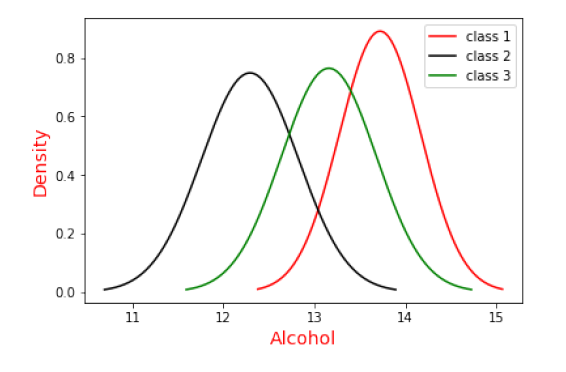
\includegraphics[width=1\textwidth]{dsc_255_hw3_q3.png} 
\caption{Estimate of confusion matrix for orginal data and normalized data using leave-one-out cross-validation (LOOCV) and 1-NN classification with Euclidean distance.}
    
\end{figure}

\begin{enumerate}[label=(a)]
    \item x has mean 2 and standard deviation 1, y has mean 2 and standard deviation 0.5, and the
correlation between x and y is -0.5.
\end{enumerate}
\begin{enumerate}[label=(b)]
    \item x has mean 1 and standard deviation 1, and y is equal to 2.
\end{enumerate}

\end{document}